\documentclass[12pt,a4paper,titlepage]{article}
\usepackage[utf8]{inputenc}
\usepackage{polski}
\usepackage{listings}
\usepackage{graphicx}
\usepackage{xcolor}
\usepackage{minted}
\usepackage{amsmath}
\usepackage{caption}
\usepackage{url}
 
\setminted{
    linenos=true,
    autogobble,
    breaklines,
    frame=lines,
    framerule=1pt,
    framesep=10pt
}

\newenvironment{longlisting}{}{}
 
\DeclareCaptionType{myequation}[][Równanie parametryczne]
\captionsetup[myequation]{labelformat=empty}

\makeatletter
\newcommand{\linia}{\rule{\linewidth}{0.4mm}}
\renewcommand{\maketitle}{\begin{titlepage}
    \vspace*{1cm}
    \begin{center}\small
    Politechnika Wrocławska\\
    Wydział Elektroniki\\
    Technologie sieciowe
    \end{center}
    \vspace{3cm}
    \noindent\linia
    \begin{center}
      \LARGE \textsc{\@title}
         \end{center}
     \linia
    \vspace{0.5cm}
    \begin{flushright}
    \begin{minipage}{7cm}
    \textit{\small Autor:}\\
    \normalsize \textsc{\@author} \par
    \end{minipage}
    \vspace{5cm}

     {\small wtorek, 07\textsuperscript{30}-9\textsuperscript{0} TN}\\
        Dr inż. Przemysław Ryba
     \end{flushright}
    \vspace*{\stretch{6}}
    \begin{center}
    \@date
    \end{center}
  \end{titlepage}%
}
\makeatother
\author{Grupa 7\\
        Justyna Skalska, 225942}
\title{Raport z laboratorium 1}

\begin{document}
\maketitle

\section{Opis firmy}

Zgodnie z danymi dla grupy nr 7, w analizowanej firmie pracuje {\bfseries 40 }osób. Pracownicy przez {\bfseries 20\%} czasu przeglądają strony WWW. Na {\bfseries 4} stacjach przez cały dzień jest uruchomione radio internetowe, a na jednej stacji TV. Wszyscy pracownicy do komunikacji wykorzystują komunikator Slack oraz pocztę elektroniczną. {\bfseries 3} razy w tygodniu odbywają się dwugodzinne wideokonferencje, w których uczestniczą {\bfseries 3} osoby. Administrator pobiera łatki korzystając z FTP, uaktualnienia, nowe wersje oprogramowania. Administrator raz w tygodniu przesyła pełny backup BD na zdalny serwer a codziennie backup 1/5 danych. Rozmiar BD to {\bfseries 10GB}.

\section{Opis sposobów generowania ruchu}
Do symulacji ruchu generowanego przez radio internetowe wykorzystałam stronę \url{http://radioluz.pwr.edu.pl/} i znajdujące się tam radio, jako telewizję internetową wybrałam \url{https://www.netflix.com}. Poczta elektroniczna, z której skorzystałam, to aplikacja Mail na MacOS z odświeżaniem skrzynki co minutę, wideokonferencję przeprowadziłam korzystając z wideorozmowy w aplikacji Google Hangouts, a do symulacji przeglądania stron WWW - weszłam na portal \url{https://www.onet.pl/}, otworzyłam kilka artykułów i przejrzałam je tak, aby częściowo załadowały się materiały wideo zmieszczone w artykułach. 

\section{Analiza logów oraz wyznaczenie ruchu i przepustowości łącza dla firmy}

Pomiary dla każdej z usług były prowadzone przez około 5 minut i były to jedyne uruchomione przeze mnie usługi internetowe na komputerze. Po 5 minutach zatrzymywałam przechwytywanie pakietów w programie Wireshark i otwierałam okno Conversations. Po posortowaniu wyświetlonych danych według malejącej ilości przesłanych pakietów, na górze listy pojawiały się statystyki dla sprawdzanej usługi.

\vspace{1cm}

\begin{figure}[H]
  \centering
    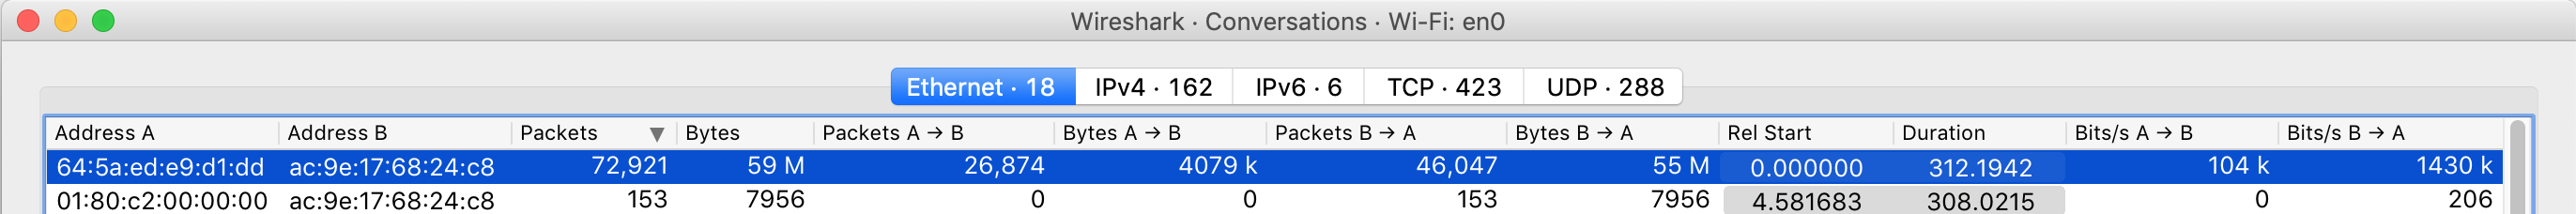
\includegraphics[width=14cm]{www-short.png}
    \caption{Obciążenie łącza podczas przeglądania stron WWW}
    \label{fig:www}
\end{figure}

Z rysunku \ref{fig:www} można odczytać, że w ciągu 5 minut zostało przesłanych 59MB, z czego 55MB zostały pobrane z sieci, a 4.1MB wysłane do sieci. Według wyliczeń programu, daje to pobieranie na poziomie 1430kb/s i wysyłanie 104kb/s.

\vspace{1cm}
\begin{figure}[H]
  \centering
    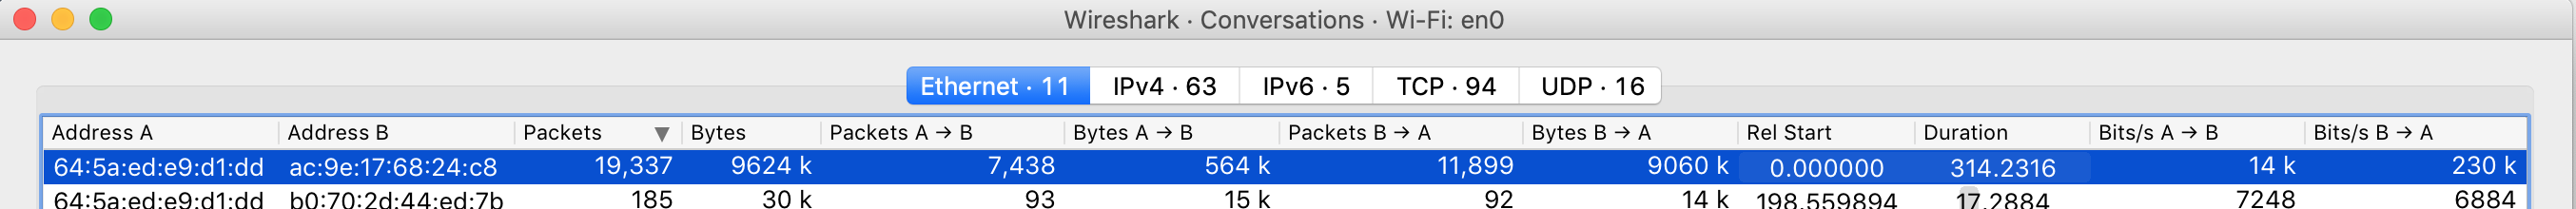
\includegraphics[width=14cm]{radio-short.png}
    \caption{Obciążenie łącza podczas słuchania radia internetowego}
    \label{fig:radio}
\end{figure}

Według danych na rysunku \ref{fig:radio}, średnia prędkość ściągania podczas pięciominutowej próby wyniosła 230kb/s, a prędkość wysyłania - 14kb/s. Odpowiadało to ściągnięciu 9,06MB i wysłaniu 564kB danych.

\vspace{1cm}
\begin{figure}[H]
  \centering
    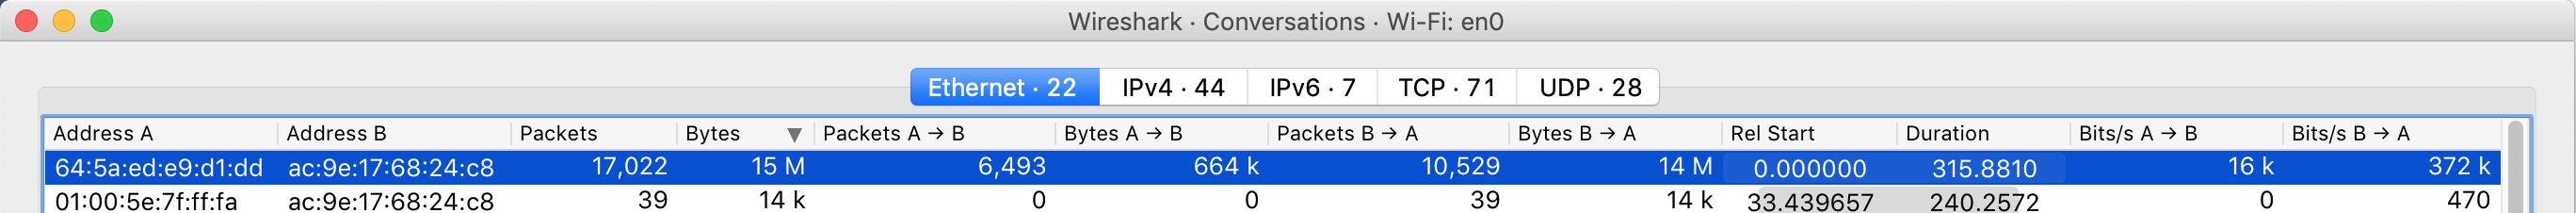
\includegraphics[width=14cm]{tv-short.png}
    \caption{Obciążenie łącza podczas oglądania telewizji internetowej}
    \label{fig:tv}
\end{figure}

Oglądanie telewizji internetowej wiązało się z przesłaniem 14MB danych przy prędkości pobierania 372kb/s i wysyłania 16kb/s.

\vspace{1cm}
\begin{figure}[H]
  \centering
    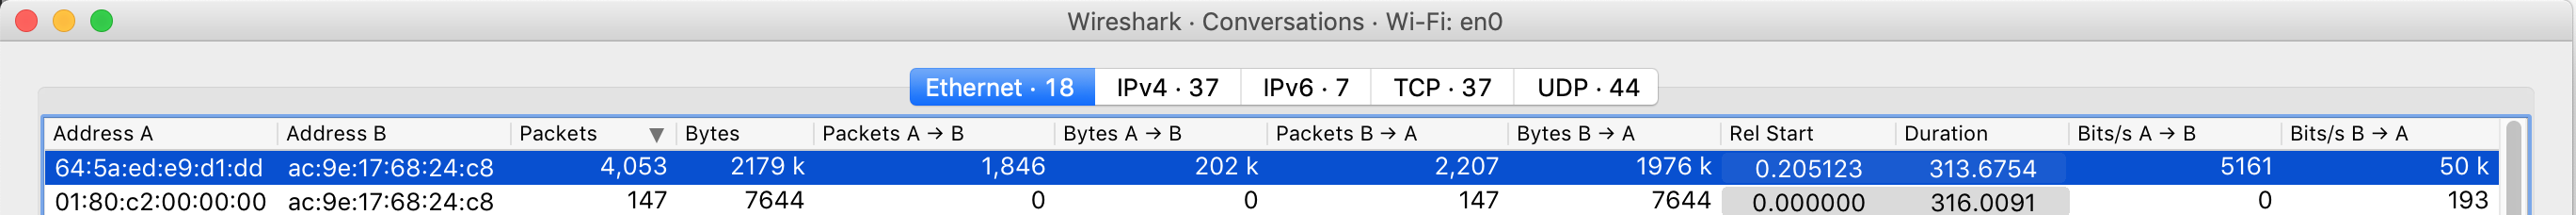
\includegraphics[width=14cm]{poczta-short.png}
    \caption{Obciążenie łącza podczas korzystania z poczty elektronicznej}
    \label{fig:poczta}
\end{figure}

Średnia przepustowość w czasie pomiarów na poziomie 50kb/s pobierania i 5kb/s wysyłania odpowiadała ściągnięciu 1,98MB i wysłaniu 202kB.

\vspace{1cm}
\begin{figure}[H]
  \centering
    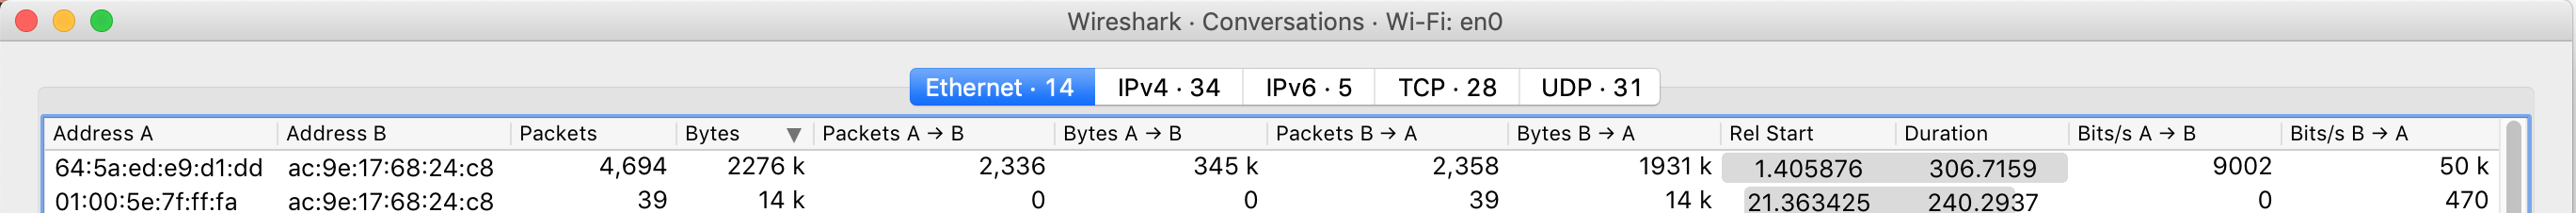
\includegraphics[width=14cm]{message.png}
    \caption{Obciążenie łącza podczas korzystania z komunikatora tekstowego}
    \label{fig:disco}
\end{figure}

Podczas spokojnej rozmowy dwóch osób, średnia prędkość ściągania i wysyłania wyniosła, odpowiednio, 9kb/s i 50kb/s. Przełożyło się to na 345kB pobranych i 1931kB wysłanych danych w ciągu 5 minut.

\vspace{1cm}
\begin{figure}[H]
  \centering
    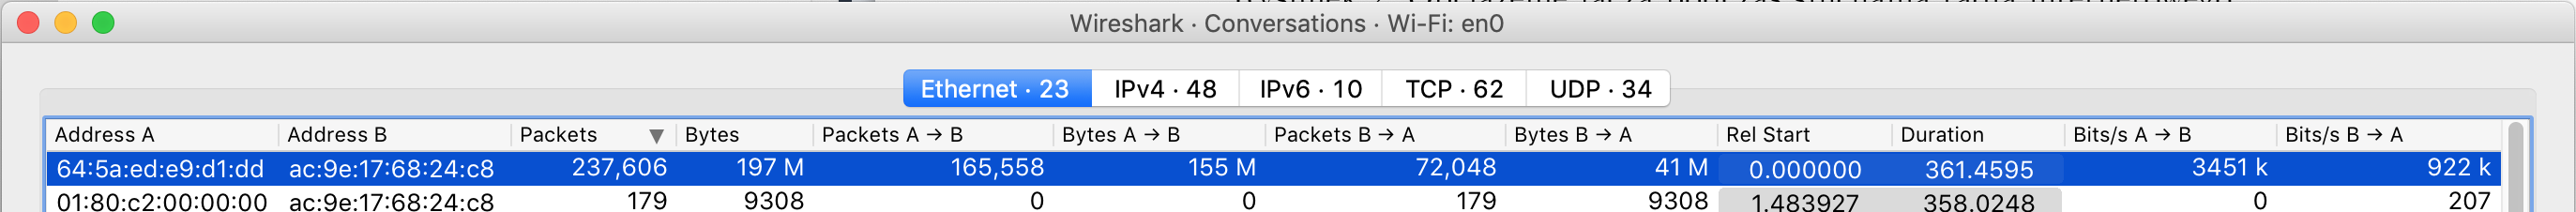
\includegraphics[width=14cm]{wideo.png}
    \caption{Obciążenie łącza podczas wideokonferencji}
    \label{fig:wideo}
\end{figure}

W ciągu 5 minut wideorozmowy dwóch osób zostało pobrane 41MB danych i wysłane 155MB. Oznacza to, że średnia przepustowość pobierania wyniosła 922kb/s, a wysyłania - 3451kb/s.
\vspace{3cm}

Codzienne przesyłanie na zdalny serwer kopii zapasowej 1/5 danych bazy danych to konieczność wysłania 2GB danych. Zakładając, że dane mają zostać wysłane w ciągu 1 godziny, wymagana prędkość wysyłania to około 0,6Mb/s. Jednocześnie zakładam, że przesłanie pełnego backupu bazy danych może trwać 5 godzin, aby obciążenie łącza podczas przesyłania kopii zapasowych dowolnej wielkości nie wymagało większej przepustowości niż 0,6Mb/s. 

\vspace{1cm}
Wymagane przepustowości dla każdej usługi liczy się mnożąc liczbę użytkowników przez przepustowości dla jednego użytkownika. Wyjątkiem jest wideokonferencja, dla której obciążenie łącza dla jednego użytkownika liczy się przez wymnożenie prędkości pobierania przez liczbę osób w wideokonferencji pozostawiając wysyłanie bez zmian, a żeby wyznaczyć całkowitą przepustowość w firmie - wynik mnoży się przez ilość osób w rozmowie. Dzieje się tak, ponieważ połączenie jest realizowane za pośrednictwem serwera, przez co jeden użytkownik wysyła dane tylko od siebie, ale pobiera od wszystkich pozostałych rozmówców.
\vspace{1cm}

Przepustowości wymagane przez dane usługi w skali całej firmy (pobieranie/wysyłanie):
\begin{itemize}
    \item Przeglądanie stron WWW - 57200kb/s, 4160kb/s,
    \item Słuchanie radia internetowego - 920kb/s, 56kb/s,
    \item Oglądanie telewizji internetowej - 372kb/s, 16kb/s,
    \item Korzystanie z poczty elektronicznej - 2000kb/s, 200kb/s,
    \item Korzystanie z komunikatora tekstowego - 360kb/s, 200kb/s,
    \item Wideokonferencje - 8298kb/s, 10353kb/s,
    \item Wysyłanie kopii zapasowej - 0kb/s, 512kb/s.
\end{itemize}

\section{Odpowiedzi na pytania}

\begin{enumerate}
\item Które usługi mają profil ruchu symetryczny, a które asymetryczny?

\vspace{0.2cm}
Symetryczny: chat, rozmowa wideo, wgrywanie/pobieranie plików przez FTP

\vspace{0.1cm}
Asymetryczny: radio, telewizja/oglądanie filmików, przeglądanie stron internetowych

\item W jakich przypadkach w firmie niezbędne jest symetryczne łącze do Internetu? 

\vspace{0.2cm}W przypadkach kiedy firma potrzebuje większych prędkości na upload. Przykłady: częste wideokonferencje, przesyłanie dużych plików pomiędzy pracownikami, własne serwery.


\item Co to jest CIR? 

\vspace{0.2cm}
Committed Information Rate - minimalna przepływowość, którą usługodawca gwarantuje użytkownikowi niezależnie od zakłóceń, liczby innych użytkowników w sieci itp.


\item Czy najważniejszym parametrem dla usługi sieciowej jest pasmo (przepustowość)? 

\vspace{0.2cm}
Niezawodność i dostępność są ważniejsze. Firma może wybrać łącze z mniejszą przepustowością jeśli usługodawca zapewni gwarancję dostępności usług.


\item Jakie usługi sieciowe wymagają także zapewnienia innych parametrów sieci (wymienić te parametry)? 

\vspace{0.2cm}
Jeśli firma chce mieć własny serwer - może potrzebować statycznego IP, Firewall itp. W przypadku pracy z urządzeniami bezprzewodowymi jest niezbędne zapewnienie usługi Wi-Fi.


\item Czy cena za łącza Internetowe rośnie liniowo wraz z przepustowością tego łącza? 

\vspace{0.2cm}
W ofertach takich dostawców jak Vectra i Multimedia, im większa jest przepustowość - tym mniej wzrasta cena. Innymi słowy, różnica w cenie między niższymi przepustowościami (150 i 300 Mb/s) jest większa niż różnica w cenie między wysokimi przepustowościami (600 i 900 Mb/s).
\end{enumerate}

\section{Podsumowanie}

Uwzględniając powyższe uwagi, minimalne wymagane prędkości ściągania i wysyłania w firmie wynoszą 69,15Mb/s i 15,50Mb/s. Wybrane łącze powinno zapewniać minimalną przepustowość na poziomie 70-80Mb/s ściągania i 16-17Mb/s wysyłania danych.

\vspace{0.5cm}
Ze względu na brak informacji w internecie o ofertach dla klientów biznesowych (wszystkie sprawdzone przeze mnie firmy firmy proszą o kontakt - oferty są spersonalizowane), nie jest możliwe wybranie konkretnego dostawcy usług internetowych.

\vspace{0.5cm}
Wszystkie testowane usługi mają profil asymetryczny. Przepustowość sieci jest podstawowym parametrem usługi sieciowej, ale nie najważniejszym. Równie ważne jest zapewnienie odpowiednio niskich opóźnień transmisji (ping), bez których niemożliwe jest korzystanie z takiej usługi jak wideokonferencja, a komunikacja tekstowa może być znacznie utrudniona. W przypadku firm niezbędne jest, aby przepustowość sieci była gwarantowana przez dostawcę Internetu i nie były niższa niż określony poziom. Taką gwarantowaną przez dostawcę przepustowość nazywamy CIR.
\end{document}